% Chapter "Barndorff-Nielsen's tools on the ladder: sand, hitting times and free probability" of Volume III. Sources: misc/reviews/nick-bn/bn/bn_chapter.tex 1-356 (summary 34, tools 36-45, Upsilon 47-82, free side 84-128, sand 130-154, why sand fits 156-209, hitting times 211-228, Berg Koumandos Pedersen 230-238, Grosswald 263-289, strip 291-300, problems 302-316; positivity test 240-261 and Code 318-321 cut); report BN.md (M1 to M10 and minors); verification misc/vol3/verify/BN/results.md. 17 Nov 2026.
\label{bn:ch:bn}

This chapter, from an unrefereed note of Polson (November 2026), runs the ladder of rungs $\alpha$ through the tools of Ole Barndorff-Nielsen: hyperbolic ("sand") laws, generalised inverse Gaussian (GIG) laws as first hitting times, the $z$ distributions, processes of Ornstein and Uhlenbeck type, and, with Thorbj{\o}rnsen, the passage to free probability through the Upsilon transform. The question behind it is the one left open by Volume~I: under RH the reciprocal Xi function $\xi(\frac12)/\xi(\frac12+\sqrt u)$ is the Laplace transform of the clock variable $T=\sum_{\gamma>0}\mathrm{Exp}(\gamma^2)$, a hitting time. Can the process be built without the zeros?

Much of the Upsilon and free material is already in Volume~I and is cited, not reprinted. The Upsilon inverse $k(v)=\widetilde U((0,1/v])$ is Proposition~\ref{prop:wigfree:ups}(b). The Dickman form of the preimage under RH is Theorem~\ref{thm:wigfree:clock}(c) and the paragraph after its proof. The free cumulant reading on the line, with its converse, is Proposition~\ref{tx2:prop:free}. Positivity of the Fourier transform of $\xi(\frac12)/\xi(\frac12+t)$ is Theorem~\ref{bs:thm:gpos}. What this chapter adds is the following.
\begin{enumerate}
\item The rung form of the Upsilon preimage, with canonical function the argument of $\xi$ along the rung (Section~\ref{bn:sec:ups}, proved), and where the primes sit in it.
\item A free Euler product for $\sigma>1$ with an atom at the origin that disappears at $\sigma=1.47446$, and the free gamma law at $\sigma=1$ (Section~\ref{bn:sec:free}; the atom is proved only in outline, the rest is proved).
\item The Thorin measure of a GIG law, one atom plus a sea of constant density, and with it an explanation of why hyperbolic laws fit the two Brownian side laws of the book (Sections~\ref{bn:sec:sand} and~\ref{bn:sec:sea}; the fits are computed).
\item P\'olya's approximant to $\Xi$ as the signed half logarithm of a GIG hitting time (Section~\ref{bn:sec:hit}, proved).
\item A reading of Grosswald's work on the Taylor coefficients of $\xi$ in the language of the Thorin atoms, Bernoulli's method for the first zero, and the modified zeta functions of Grosswald and Schnitzer, whose rung density goes negative (Section~\ref{bn:sec:grosswald}, computed).
\end{enumerate}
None of this proves RH or constructs the process from the primes. In every construction the input is the zeros or the argument of $\xi$. Status words follow the book: proved, computed (floating point), heuristic, open. The Thorin measures of the rungs are written in the book's chart $u=w^2$, with atoms $\gamma^2$. The sand sections use the Brownian time $H=2T$, whose Thorin atoms are $\gamma^2/2$, because that is the natural parametrisation of the GIG laws; measures in the variable $r=\sqrt{2z}$ are the same in both.

\section{The tools}\label{bn:sec:tools}
Statements are quoted from the papers in the references. The Bercovici and Pata bijection $\Lambda_{\rm BP}$ and the Upsilon transform are in Section~\ref{sec:wigfree:bp}, with the identity~\eqref{eq:wigfree:bnt}. The other tools are these.
\begin{itemize}
\item \textit{Sand.} A hyperbolic law has log density a hyperbola, $-\varkappa\sqrt{\delta^2+x^2}+\beta x$ up to a constant, hence linear asymptotes. It was introduced for the size distribution of windblown sand, after Bagnold, and it is a normal variance and mean mixture with a GIG mixing law \cite{BN77}.
\item \textit{GIG.} The GIG laws are infinitely divisible \cite{BNH77} and are generalised gamma convolutions \cite{Halgreen79}. Every GIG law with nonpositive index is the first hitting time of $0$ of a time homogeneous diffusion on $[0,\infty)$ \cite{BBH78}.
\item \textit{$z$ distributions.} They are normal variance and mean mixtures whose mixing law is an infinite convolution of exponential laws \cite{BNKS82}. The zeta law as an infinitely divisible law is Section~\ref{mw:sec:khinchin}.
\item \textit{OU processes.} Every self decomposable law is the stationary law of a process of Ornstein and Uhlenbeck type $\mathrm dX=-cX\,\mathrm dt+\mathrm dL(ct)$ driven by a L\'evy process, and superpositions of such processes are again stationary \cite{BNS01,BN01}.
\item \textit{Upsilon and free.} The image of the infinitely divisible laws under $\Upsilon$ is the class of Goldie, Steutel and Bondesson and that of the self decomposable laws is the Thorin class \cite{BNMS06,BNT06}. The bijection $\Lambda_{\rm BP}$ keeps self decomposability, with free L\'evy and free OU processes on the other side \cite{BNT02}, and $\Lambda_{\rm BP}(\mu)$ is the limiting spectral law of a random matrix model \cite{BenaychGeorges05,CabanalDuvillard05}.
\end{itemize}

\section{Upsilon on the ladder}\label{bn:sec:ups}
Recall the uncompensated Thorin measure of rung $\alpha$. As a measure in $r$ it has density $\frac1\pi\Re\,\xi'/\xi(\alpha+ir)$, so that its mass on $[0,R]$ is $\frac1\pi\arg\xi(\alpha+iR)$ (Theorem~\ref{thm:poisson}). Throughout the chapter we quote values of $\Re\,\xi'/\xi$, which is $\pi$ times the density. When the density is nonnegative, which is every $\alpha>1$ unconditionally and every $\alpha>\frac12$ under RH,
\[
\frac{\xi(\alpha)}{\xi(\alpha+\sqrt u)}=\exp\Bigl(-\int\log\bigl(1+\tfrac uz\bigr)\,\mu^\circ_\alpha(\mathrm dz)\Bigr)=\mathbb E\,e^{-uX_\alpha},
\]
with $X_\alpha$ a generalised gamma convolution without drift.
\begin{proposition}[the rung as an Upsilon image, proved]\label{bn:prop:ups}
On such a rung $X_\alpha=\Upsilon(Z_\alpha)$ in law, where $Z_\alpha$ is the self decomposable law on $(0,\infty)$ with L\'evy density $k_\alpha(y)/y$ and
\[
k_\alpha(y)=\frac1\pi\arg\xi\bigl(\alpha+i/\sqrt y\bigr).
\]
Equivalently $X_\alpha$ has the law of $\int_0^1\log(1/t)\,\mathrm dZ_\alpha(t)$ for the subordinator $Z_\alpha$ with $Z_\alpha(1)\sim Z_\alpha$.
\end{proposition}
\begin{proof}
This is Proposition~\ref{prop:wigfree:ups}(b) with the rung Thorin measure, whose mass on $r\le R$ is $\frac1\pi\arg\xi(\alpha+iR)$, with $R=y^{-1/2}$ (the book's atom $\gamma^2$ sits at $r=\gamma$). There is no drift, because $1/\xi(\alpha+\sqrt u)$ decays more slowly than any $e^{-du}$.
\end{proof}
On the line under RH the preimage is $\sum_{\gamma>0}D_\gamma/\gamma^2$ with independent Dickman variables $D_\gamma$ (Theorem~\ref{thm:wigfree:clock}(c) and the paragraph after its proof); $\Upsilon$ turns the indicator of an interval, which is the Dickman law, into an exponential law. On a rung $Z_\alpha$ is a continuous mixture of scaled Dickman laws: its L\'evy density is $\int\mu^\circ_\alpha(\mathrm dz)\,\mathbf 1_{(0,1/z)}(y)/y$.
\begin{corollary}[RH as monotonicity: Lagarias' criterion]\label{bn:cor:mono}
RH holds if and only if for every $\alpha>\frac12$ the function $R\mapsto\arg\xi(\alpha+iR)$ is nondecreasing on $R>0$, that is, if and only if every $k_\alpha$ is the canonical function of a self decomposable law.
\end{corollary}
\begin{proof}
The derivative in $R$ is $\Re\,\xi'/\xi(\alpha+iR)=\sum_\rho(\alpha-\beta)/|\alpha+iR-\rho|^2$, positive if no zero has $\beta>\alpha$ and tending to $-\infty$ as $\alpha+iR$ approaches a zero with $\beta>\alpha$ from the left.
\end{proof}
This is the criterion of Lagarias \cite{Lagarias}, as used in Section~\ref{ht:sec:frontier}. Among the many equivalents on the ladder it is the one in which the object is a single function with a name in number theory, the argument of $\xi$, and the property is the defining one of a named class of laws. For $\alpha>1$ it holds unconditionally.

\medskip\noindent\textit{Computed checks on the rung $\alpha=2$.} The quantity $\Re\,\xi'/\xi(2+ir)$ is at least $0.0691$ on $0<r\le4000$, with minimum $0.0691$ approached as $r\to0$. The integral $\int\log(1+u/r^2)\,\mu_2^\circ(\mathrm dr)$ over $0<r\le4000$ is $0.09150$, $0.22725$, $0.62648$ at $u=1,4,16$, and the tail beyond $r=4000$ adds $0.00030$, $0.00119$, $0.00475$, giving $0.09180$, $0.22844$, $0.63123$, equal to $\log\xi(2+\sqrt u)/\xi(2)$ to five digits. The canonical function at $R=10,20,30,50$ is $k_2=0.2772$, $1.6062$, $3.8059$, $9.8290$. The Dickman identity $\int_0^\infty C_D(ubx)\,e^{-x}\,\mathrm dx=-\log(1+ub)$ holds to fifteen digits at $b=0.7$, $u=1.3$, both sides being $-0.647103242058539$.

\medskip\noindent\textit{Where the primes sit.} For $\alpha>1$, with $R=y^{-1/2}$ and $\Lambda(n)$ the von Mangoldt function,
\[
k_\alpha(y)=k^\Gamma_\alpha(y)+k^{\mathrm{pole}}_\alpha(y)-\frac1\pi\sum_n\frac{\Lambda(n)}{n^\alpha\log n}\sin(R\log n),
\]
the first two terms being the arguments of $\pi^{-s/2}\Gamma(\frac s2)$ and of $s(s-1)$ along the rung. So at the level of $Z_\alpha$ the Euler product is additive in $k$, each prime power contributes a bounded oscillation, and self decomposability is a statement about the sum only: no prime term is monotone. In the strip the sum over $n$ diverges and what remains is the monotonicity question of Corollary~\ref{bn:cor:mono}.

\section{The free side}\label{bn:sec:free}
\begin{proposition}[the rung as a free cumulant transform, proved]\label{bn:prop:free}
On a rung with nonnegative Thorin density, in particular for every $\alpha>1$ and, under RH, every $\alpha>\frac12$, for $s>0$
\[
\log\frac{\xi(\alpha)}{\xi(\alpha+\sqrt s)}=-\Psi_{X_\alpha}(s)=\mathcal C_{\Lambda_{\rm BP}(Z_\alpha)}(-s).
\]
The law $\Lambda_{\rm BP}(Z_\alpha)$ is freely self decomposable, the stationary law of a free OU process and the limiting spectral law of a random matrix model.
\end{proposition}
\begin{proof}
Proposition~\ref{bn:prop:ups} and Proposition~\ref{prop:wigfree:ups}(a), which gives $\mathcal C_{\Lambda_{\rm BP}(\mu)}(-s)=-\Psi_{\Upsilon(\mu)}(s)$ for $s>0$; the rest is quoted from \cite{BNT02,BenaychGeorges05,CabanalDuvillard05}.
\end{proof}
On the line this is Proposition~\ref{tx2:prop:free}, which also proves the converse. So there is a matrix ensemble whose limiting spectral law has $-\log\xi$ along the rung for free cumulant transform. It is not the ensemble of the Montgomery and Dyson picture \cite{Montgomery73,Dyson62}: there the zeros are the eigenvalues, here they are the atoms of the Thorin measure of the classical preimage. The ensemble is defined from $k_\alpha$, that is from $\arg\xi$.

Where the Euler product converges the free side can be built from the primes.
\begin{theorem}[free Euler product]\label{bn:thm:feuler}
Let $\sigma>1$ and let $N_\sigma$ have the zeta law, so that $\log N_\sigma$ is compound Poisson with L\'evy measure $\sum_nc_n\delta_{\log n}$, $c_n=\Lambda(n)n^{-\sigma}/\log n$. Then
\[
\Lambda_{\rm BP}(\log N_\sigma)=\mathop{\boxplus}_{p,k}\;\mathrm{MP}\bigl(p^{-k\sigma}/k;\,k\log p\bigr),
\]
a free convolution of free Poisson (Marchenko and Pastur) laws with rates $p^{-k\sigma}/k$ and jumps $k\log p$. Its $R$ transform is $R(w)=\sum_nc_n\log n/(1-w\log n)$, its mean is $-\zeta'/\zeta(\sigma)$, and its free cumulant transform is a Laplace average of $\log\zeta$ along a ray,
\[
\sum_nc_n\Bigl(\frac1{1-iz\log n}-1\Bigr)=\int_0^\infty\log\frac{\zeta(\sigma-izx)}{\zeta(\sigma)}\,e^{-x}\,\mathrm dx.
\]
All of this is proved. In addition it has an atom at the origin of mass $1-\log\zeta(\sigma)$ if $\zeta(\sigma)<e$, that is $\sigma>1.47446$, and no atom otherwise (proved in outline only, see the sketch), while the classical law has the atom $1/\zeta(\sigma)$ for every $\sigma>1$.
\end{theorem}
\begin{proof}
$\Lambda_{\rm BP}$ keeps the L\'evy measure, and the free law with L\'evy measure $c\,\delta_a$ is the free Poisson law with $R(w)=ca/(1-aw)$; $R$ is additive. The cumulant identity is $C_{\Upsilon(\mu)}(z)=\int_0^\infty C_\mu(zx)e^{-x}\,\mathrm dx$ with $C_\mu(z)=\log\zeta(\sigma-iz)/\zeta(\sigma)$, continued from the negative imaginary axis as in Theorem~\ref{thm:wigfree:clock}(b), where~\eqref{eq:wigfree:bnt} is stated for real argument.
\end{proof}
\begin{remark}[sketch of the atom]
Write $\lambda=\sum c_n=\log\zeta(\sigma)$. As $w\to\infty$, $R(w)=-\lambda/w+O(w^{-2})$, so the Cauchy transform $G$, which solves $z=1/G+R(G)$, satisfies $z\approx(1-\lambda)/G$ for large $G$, that is $G\approx(1-\lambda)/z$ near $z=0$ when $\lambda<1$. This reads off the atom on the assumption that $G$ is large near $0$. It does not prove that an atom exists when $\lambda<1$, and when $\lambda\ge1$ it only rules out this ansatz. The statement is that of the atom $\max(0,1-\lambda)$ of a free compound Poisson law whose jump law has no mass at $0$; we have not checked it against a source % UNCHECKED
and give it as a computed fact at $\sigma=2$: the atom found from the Cauchy transform is $0.5023$ against $1-\log\zeta(2)=0.5023$, while the classical atom is $0.6079$. A complete proof would use $\mu(\{0\})=\lim_{y\downarrow0}\,iy\,G(iy)$ with the subordination form of $z=1/G+R(G)$.
\end{remark}
\noindent\textit{Computed checks at $\sigma=2$,} prime powers to $10^6$ (78734 terms): total rate $0.49770023$ against $\log\zeta(2)=0.49770030$; mean $0.5699600$ against $-\zeta'/\zeta(2)=0.5699610$; the two sides of the cumulant identity at $z=0.3$ are $-0.05685599+0.13994312\,i$ and $-0.05685605+0.13994314\,i$; the atom as above; the continuous part has mass $0.4958$ on $0.02<x<6$, starts near $x=0.1$ and has its mode at $x=0.15$. The value $\sigma=1.47446$ solves $\zeta(\sigma)=e$.

At the edge of convergence the free Euler product has a limit, and the limit is the pole.
\begin{theorem}[the pole is a free gamma law, proved]\label{bn:thm:fgamma}
As $\sigma\downarrow1$, the law of $(\sigma-1)$ times a variable with law $\Lambda_{\rm BP}(\log N_\sigma)$ converges weakly to $\Lambda_{\rm BP}(\mathrm{Exp}(1))$, the free gamma law of shape one \cite{HaagerupThorbjornsen14}, with $R$ transform $R(w)=\int_0^\infty\frac{e^{-y}}{1-wy}\,\mathrm dy$, mean one and variance one.
\end{theorem}
\begin{proof}
Classically $(\sigma-1)\log N_\sigma$ converges in law to the exponential law, since $\zeta(\sigma-i(\sigma-1)t)/\zeta(\sigma)\to1/(1-it)$: this is the pole of $\zeta$. The bijection $\Lambda_{\rm BP}$ is a homeomorphism for weak convergence and commutes with dilations \cite{BP99,BNT02}.
\end{proof}
\noindent Computed (prime powers to $10^6$, the tail of the $R$ transform by the prime number theorem; % UNVERIFIED
not recomputed by the editor): the Kolmogorov distance between the scaled free Euler product and the free gamma law is $0.182$, $0.071$, $0.022$ at $\sigma=1.3$, $1.1$, $1.03$, and the means are $0.843$, $0.945$, $0.983$. So the free side reproduces the classical picture: just to the right of $\sigma=1$ the primes look like the pole, here a free gamma variable. Below $\sigma=1$ there is no free Euler product, as there is no classical one.

\begin{remark}[how the zeros would enter, heuristic]
Continued in the argument of $z$, the path $s=\sigma-izx$, $x>0$, is a ray from $\sigma$, and the Laplace average is singular when the ray meets a zero or the pole. RH would say that seen from $\sigma$ every ray through a zero ends on the line $\Re s=\frac12$. This is a restatement, recorded because the object on the left is defined by the primes alone. The log singularities at the zeros are integrable, so this is not a theorem about the transform.
\end{remark}

\section{Sand}\label{bn:sec:sand}
The book has two laws on the Brownian side, and both have log densities with linear asymptotes. Write $\widehat\zeta(s)=\pi^{-s/2}\Gamma(\frac s2)\zeta(s)$ for the completed zeta function without the factor $s(s-1)$.
\begin{proposition}[slope one half, proved]\label{bn:prop:half}
The law of $V+L$ on the critical line has density $\bigl(e^{-|x|/2}-2e^{|x|/2}\psi(e^{2|x|})\bigr)/|\widehat\zeta(\frac12)|$, with $\psi(y)=\sum_{n\ge1}e^{-\pi n^2y}$, and characteristic function $\widehat\zeta(\frac12-it)/\widehat\zeta(\frac12)$. Its log density is $-\frac{|x|}2-\log|\widehat\zeta(\frac12)|$ up to a doubly exponentially small term. This is unconditional.
\end{proposition}
\noindent This is Theorem~\ref{nf:thm:line} in other notation ($V$ here is $X$ there). The statement on the log density is immediate from the displayed density, since $\psi(e^{2|x|})$ is doubly exponentially small.
\begin{proposition}[slope $\gamma_1$, under RH]\label{bn:prop:slope}
Under RH, $\xi(\frac12)/\xi(\frac12+t)$, $t$ real, is the characteristic function of $B_H$, Brownian motion at the independent time $H=\sum_{\gamma>0}\mathrm{Exp}(\gamma^2/2)=2T$: a normal variance mixture whose mixing law is an infinite convolution of exponentials, as for the $z$ distributions, with the squares of the zeros in the place of the squares of an arithmetic progression. Its density is $\sum_{\gamma>0}a_\gamma e^{-\gamma|x|}$, so its log density has the asymptote $\log|a_1|-\gamma_1|x|$ with $\gamma_1=14.1347$ and $|a_1|=\xi(\frac12)/|\xi'(\rho_1)|=359.52$.
\end{proposition}
\noindent The function $\xi(\frac12)/\xi(\frac12+t)$ uses only the values of $\xi$ on the real axis, so its inverse Fourier transform can be computed without any hypothesis. By Theorem~\ref{bs:thm:gpos} it is positive for all real $x$ unconditionally, and the proof controls all hypothetical off line pairs of zeros at once. The consequence for this chapter stands: every statement that uses only $\xi$ on the real axis is blind to the zeros off the line, the sand fits included. Information about the zeros is on the rungs, in the argument of $\xi$.

Hyperbolic fits, in the sup norm on the density (computed; % UNVERIFIED
fitted by the draft authors, not recomputed). Here $\varkappa$ is the slope of the hyperbola:
\begin{center}
\small
\begin{tabular}{llll}
\toprule
law & $\varkappa$ & $\delta$ & error, as a fraction of the peak\\
\midrule
$V+L$, slope fixed & $0.5$ & $0.175$ & $0.0020/0.2297=0.9\%$\\
$V+L$, free & $0.507$ & $0.219$ & $0.00097/0.2297=0.4\%$\\
$B_H$, slope fixed & $14.13$ & $0.570$ & $0.0159/1.899=0.8\%$\\
$B_H$, free & $19.77$ & $0.834$ & $0.00060/1.899=0.03\%$\\
\bottomrule
\end{tabular}
\end{center}
Neither law is hyperbolic: the first differs by a theta function, and the second has the wrong slope in the bulk, where the best hyperbola has $\varkappa=19.8$, while the true asymptote, reached slowly (the density is $0.94$ of its leading term at $x=1$), has $\varkappa=\gamma_1$. But the shape is Bagnold's: a parabola at the centre and straight lines in the tails. If $B_H$ were exactly hyperbolic its mixing law would be GIG and the hitting time of Section~\ref{bn:sec:hit} would answer the question of this chapter. It is not, because $H$ is an infinite convolution of exponentials and no GIG law is.

\section{Why sand fits: one atom and a sea}\label{bn:sec:sea}
A first remark keeps the numbers honest: $B_H$ is close to normal in the bulk. Its excess kurtosis is $12\sum\gamma^{-4}/(2\sum\gamma^{-2})^2=0.209$ (sums over $\gamma>0$; computed from the Taylor coefficients of $\xi$ at $\frac12$ and from the zeros, both $0.2089$), and the normal law of the same variance already fits to $2.3\%$ of the peak. The hyperbolic law improves this by a factor of about $70$; the normal inverse Gaussian law ($0.030\%$) and the generalised hyperbolic law with free index ($0.027\%$, at index $-3.8$) do no better than the hyperbolic one ($0.031\%$). % UNVERIFIED: fit errors from the draft
\begin{theorem}[Thorin measure of a GIG law]\label{bn:thm:gig}
The GIG law with index $\lambda$ and density proportional to $y^{\lambda-1}\exp(-\frac12(\delta^2/y+\varkappa^2y))$, in the Laplace variable of $y$, has Thorin measure
\begin{align*}
U&=\max(\lambda,0)\,\delta_{\varkappa^2/2}+\delta^2g_{|\lambda|}\bigl(2\delta^2(z-\tfrac{\varkappa^2}2)\bigr)\mathbf 1_{z>\varkappa^2/2}\,\mathrm dz,\\
g_\nu(\xi)&=\frac{2}{\pi^2\xi\,\bigl(J_\nu^2(\sqrt\xi)+Y_\nu^2(\sqrt\xi)\bigr)}.
\end{align*}
As a measure in $r=\sqrt{2z}$ the continuous part has density tending to the constant $\delta/\pi$.
\end{theorem}
\begin{proof}
This is the L\'evy density of the GIG laws, known from the work of Barndorff-Nielsen and Shephard and resting on Grosswald's formula for $K_{\nu-1}/K_\nu$ \cite{Grosswald76a,Ismail77,BNS01}, read as a Laplace transform in $x$. The normalisation $\delta^2g_{|\lambda|}$ is confirmed by recovering the inverse Gaussian L\'evy density $\delta x^{-3/2}/\sqrt{2\pi}$. The constant follows from $J_\nu^2+Y_\nu^2\sim2/(\pi\sqrt\xi)$.
\end{proof}
\noindent Computed checks: $-\log\mathbb E\,e^{-uX}$ against $\int\log(1+u/z)\,U(\mathrm dz)$ agrees to nine digits or better at several parameter values: $\lambda=1$, $\delta=0.57$, $\varkappa=\gamma_1$, $u=50$ gives $2.124513492$ on both sides; $\lambda=-\frac94$, $\delta=0.9$, $\varkappa=2$, $u=3$ gives $0.5660259713$ on both sides; $\lambda=\frac12$ and $\lambda=1$, $u=5$ agree to ten digits. The density of the sea at $r=3000$ times $\pi/\delta$ is $1.00001$ for $\lambda=1$, $\delta=0.57$.
\begin{corollary}[what a hyperbolic law is]\label{bn:cor:sea}
The symmetric hyperbolic law with parameters $\varkappa,\delta$ is Brownian motion at a time whose Thorin measure is one atom of mass one at $\varkappa^2/2$ followed by a sea of asymptotically constant density $\delta/\pi$ in $r$. Among the generalised hyperbolic laws with $\beta=0$ and positive index $\lambda$ the Thorin measure begins with an atom of mass $\lambda$, so the hyperbolic law is the one with mass one.
\end{corollary}
Compare with $B_H$, whose time has the Thorin measure $\sum_{\gamma>0}\delta_{\gamma^2/2}$: a simple atom at the first zero followed by atoms of density $\frac1{2\pi}\log\frac r{2\pi}$ in $r$. So the hyperbolic law with slope $\gamma_1$ is the reciprocal Xi function with the first zero kept and all the other zeros melted into a sea of constant density. The fitted $\delta=0.570$ gives the density $\delta/\pi=0.181$, and the zeros have this density at the height $2\pi e^{2\delta}=19.65$, between the first and second zeros: the fit chose the local density of zeros. The same reading applies to $V+L$ on the line: the atom of its hyperbolic fit, at $\varkappa^2/2=\frac18$ with mass one, is the Laplace variable $L$ of the two poles, and the thin sea ($\delta=0.175$) stands in for $V$.

The sea is also where the hyperbolic laws fail. Their Thorin mass on $[0,R]$ grows like $\delta R/\pi$ and that of the zeros like $\frac R{2\pi}\log\frac R{2\pi e}$ (computed; the hyperbolic row was reproduced independently):
\begin{center}
\small
\begin{tabular}{lrrrrr}
\toprule
$R$ & $20$ & $30$ & $50$ & $100$ & $200$\\
\midrule
hyperbolic, slope $\gamma_1$ & $3.33$ & $5.56$ & $9.46$ & $18.71$ & $36.95$\\
zeros $N(R)$ & $1$ & $3$ & $10$ & $29$ & $79$\\
smooth count & $1.38$ & $3.56$ & $9.42$ & $29.00$ & $79.19$\\
\bottomrule
\end{tabular}
\end{center}
No generalised hyperbolic law can be exact, and the obstruction is the logarithm in the density of zeros. The Bessel zeros behind the GIG laws are asymptotically an arithmetic progression, as are the poles behind the $z$ distributions; the zeros of $\xi$ are not.

This suggests the right sand for $\xi$: keep the first $m$ zeros as atoms and replace the rest by the logarithmic sea, of density $\frac1{2\pi}\log\frac r{2\pi}$ in $r$ beyond the height $R_m$ at which the smooth count equals $m$. The sea is the smooth part of the counting function, that is, the Gamma factor. The resulting laws, compared with $B_H$ in the sup norm as a fraction of the peak (computed; % UNVERIFIED
only $R_0=9.68$ and $R_1=17.85$ were checked by the referee):
\begin{center}
\small
\begin{tabular}{lrrrrrr}
\toprule
atoms $m$ & $0$ & $1$ & $2$ & $5$ & $10$ & $30$\\
\midrule
$R_m$ & $9.68$ & $17.85$ & $23.17$ & $35.47$ & $51.73$ & $102.26$\\
error & $0.69\%$ & $0.25\%$ & $0.011\%$ & $0.038\%$ & $0.0020\%$ & $0.0009\%$\\
\bottomrule
\end{tabular}
\end{center}
With no zeros at all, the Gamma factor alone gives $0.7\%$. With two zeros the error is $0.011\%$, below every generalised hyperbolic fit, and it is not monotone in $m$ because $R_m$ falls in a gap or near a zero; the last entry is at the accuracy of the quadrature. These laws are defined only when the first $m$ zeros are real, which is known for every $m$ that occurs here; each is then a generalised gamma convolution by construction, and as $m$ grows they converge to $B_H$ under RH.
\begin{figure}[t]
\centering
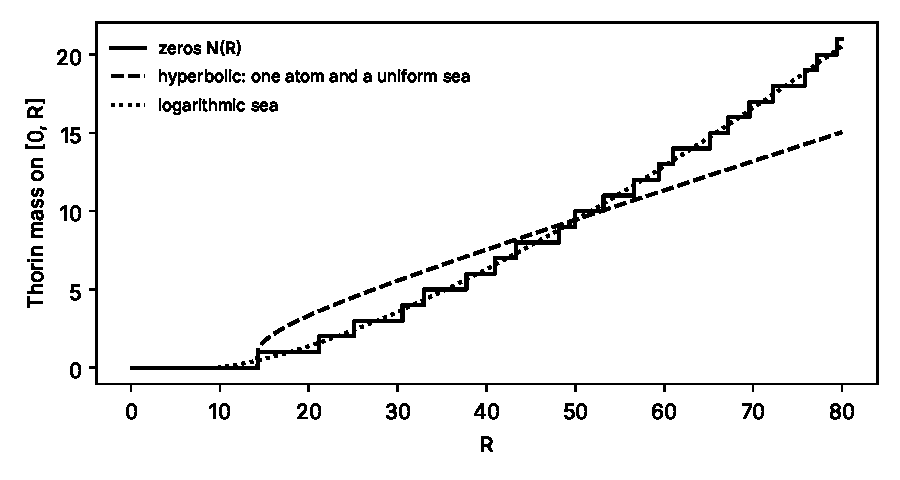
\includegraphics[width=0.8\textwidth]{fig/v3/bn_sea.pdf}
\caption{Thorin mass on $[0,R]$, as measures in $r$: the zeros, the hyperbolic law with slope $\gamma_1$ (one atom and a uniform sea), and the logarithmic sea.}\label{bn:fig:sea}
\end{figure}
% The draft figure fig_bn.pdf (hyperbolic fits of the two side laws, free Euler product density) is not included: its fitted curves rest on the unverified fit table above, and it must be redrawn from verified fits before it is used.

\medskip\noindent\textit{Are the hyperbolic laws valuable for the programme?} As descriptions, yes: Corollary~\ref{bn:cor:sea} explains in one line why a two parameter law reproduces the reciprocal Xi function so closely, and the GIG law has an explicit Thorin measure, hitting time and density. As a route to the zeros, no: a GIG sea has constant density, and every member of the family beyond the first atom is blind to where the zeros are. The $z$ distributions and the Gamma factor are more valuable than the hyperbolic laws, because they supply the right sea.

\section{Hitting times: GIG, P\'olya, and processes for $T$}\label{bn:sec:hit}
\begin{proposition}[P\'olya's approximant is a hitting time, proved]\label{bn:prop:polya}
P\'olya's function $\Xi^*(z)=4\pi^2\bigl(K_{\frac94+\frac{iz}2}(2\pi)+K_{\frac94-\frac{iz}2}(2\pi)\bigr)$ \cite{Polya}, which has only real zeros (Proposition~\ref{pol:prop:bessel}), is a constant times the characteristic function of
\[
V^*=\tfrac{\varepsilon}{2}\log S,
\]
where $\varepsilon=\pm1$ is a fair sign and $S$ is an independent GIG variable with index $-\frac94$ and density proportional to $y^{-13/4}\exp(-\pi(y+1/y))$. By the theorem of Barndorff-Nielsen, Bl{\ae}sild and Halgreen \cite{BBH78}, $S$ is the first hitting time of $0$ of a diffusion on $[0,\infty)$.
\end{proposition}
\begin{proof}
$K_\nu(\omega)=\frac12\int e^{\nu v-\omega\cosh v}\,\mathrm dv$, so $K_{\frac94+\frac{iz}2}(2\pi)$ is a constant times the Fourier transform at $z$ of the law of $\frac12\log Y$, $Y$ of GIG type with index $\frac94$ and density proportional to $y^{5/4}e^{-\pi(y+1/y)}$; and $1/Y$ has index $-\frac94$.
\end{proof}
So on the side of $V$ hitting times were present from the start: P\'olya's approximant is the signed half logarithm of one diffusion hitting time, and by Biane, Pitman and Yor \cite{BPY01} the function $2\xi(s)$ itself is a Mellin transform of a variable built from two independent hitting times of the three dimensional Bessel process. The question of this chapter is on the other side, for the Wald partner. Barndorff-Nielsen's tools give three processes for it.
\begin{itemize}
\item \textit{A superposition of OU processes.} The exponential law of rate $\theta$ is the stationary law of the OU process driven by a compound Poisson process of unit rate with exponential jumps of rate $\theta$. Under RH the superposition over the zeros, one such process for each $\gamma$ with $\theta=\gamma^2$, is stationary with law $T$. The L\'evy density of $T$ is $u(x)/x$ with $u(x)=\sum_{\gamma>0}e^{-\gamma^2x}$, the heat trace of the zeros.
\item \textit{A stochastic integral.} $T=\int_0^1\log(1/t)\,\mathrm dZ(t)$ with $Z$ the subordinator with $Z(1)=\sum_\gamma D_\gamma/\gamma^2$ of Theorem~\ref{thm:wigfree:clock}(c) and the paragraph after its proof.
\item \textit{A free OU process and a matrix model} for $\Lambda_{\rm BP}(Z(1))$, by Proposition~\ref{bn:prop:free}.
\end{itemize}
Each is a process whose marginal or stationary law gives the reciprocal Xi function, and each is defined from the zeros. They answer the question ``is there a process'' and not the question ``can it be built from arithmetic''. The Krein string of the earlier chapters is in the same position.

\section{A paper of Berg, Koumandos and Pedersen}\label{bn:sec:bkp}
Their paper on Nielsen's beta function \cite{BKP19} belongs to the same school and bears on the programme at four points. The statement numbers below are those of our reading of the paper.
% UNCHECKED: theorem, proposition and example numbers of BKP19 as given in the draft; only the arXiv record was checked by the draft authors.
\begin{itemize}
\item \textit{A weaker rung.} Their Theorem 2.1, due to Kristiansen \cite{Kristiansen94}, says that a generalised Stieltjes function of order $2$, $\int\mu(\mathrm dt)/(x+t)^2$, is logarithmically completely monotone, that is, an infinitely divisible Laplace transform; equivalently a density $x\,g(x)$ with $g$ completely monotone is infinitely divisible. The Thorin condition asks that $-(\log\phi)'$ be a Stieltjes function of order $1$. So order $2$ for $\phi$ itself is a different and often checkable sufficient condition for infinite divisibility, though not for the Thorin class. It does not apply to $T$, whose density vanishes to infinite order at $0$ and so is not of the form $x\,g(x)$.
\item \textit{Entire functions with negative zeros.} Their Proposition 4.4 states that for an entire function $f$ of genus one with only negative zeros $-a_n$ (the proof covers genus zero), $\log\frac{f(x+a)f(x+b)}{f(x)f(x+a+b)}$ is of order $2$ with representing density $\chi_{(0,a)}*\chi_{(0,b)}*\sum\delta_{a_n}$. In the variable $u$ the function $f(u)=\xi(\frac12+\sqrt u)/\xi(\frac12)$ is such a function exactly under RH, with $a_n=\gamma_n^2$. So second differences of $\log\xi$ in $u$ have a positive representing density, the comb of the zeros smoothed by two boxes: a finite difference form of the Thorin measure. It is a consequence of RH, and the hypothesis of the proposition is RH.
\item \textit{The Gamma factor.} Their Example 6.5 treats $\int_0^\infty e^{-xt}(1+e^{-t})^{-a}t^{\lambda-1}\,\mathrm dt$ for $0<a\le1$, which is the Mellin family of Chapter~\ref{ml:ch:mellin} with $a=2\lambda$ at the tilt $x=\lambda$, and their Corollary 1.4 and Remark 2.5 give the infinite divisibility of $1/\cosh$ and of $t/\sinh$ on the half line. These are unconditional statements about the Gamma factor and complement the Mellin chapter, where the same integrals were studied in the other variable.
\item \textit{Hamburger's formula.} Their Remark 2.2 recalls that $x^{-1}\prod_{k\le n}(1+x^2/(k\pi)^2)^{-1}$ is a constant times $\int_0^\infty e^{-xt}(1-\cos\pi t)^n\,\mathrm dt$. For $n=1$ both sides are $\pi^2/(x(x^2+\pi^2))$ up to the constant. This is the $2\sin^2$ kernel raised to the power $n$: for zeros in arithmetic progression the reciprocal of $x$ times the partial product is the Laplace transform of a power of $2\sin^2(\pi t/2)$, a positive periodic function. The positivity uses the progression. For the zeros of $\xi$ the corresponding function is not periodic and not positive, and the book's lemma replaces the power by a mixture.
\end{itemize}
The paper is a source of tools and of unconditional facts about the Gamma factor. It contains nothing that locates a zero, since in each result the real zeros are a hypothesis.

\section{Grosswald and the Taylor coefficients of $\xi$}\label{bn:sec:grosswald}
\textit{Grosswald's paper of 1966.} % UNCHECKED: Grosswald, Illinois J. Math. 10 (1966), 9 to 23, was not opened; its content is stated from the citing literature (introduction of CNV86).
As reported in the citing literature \cite{CNV86}, Grosswald \cite{Grosswald66} generalised a formula of Hayman \cite{Hayman56} for the Taylor coefficients of an admissible entire function, applied it to $\xi$ to obtain the asymptotic behaviour of the Taylor coefficients at $s=\frac12$, and deduced from it the Tur\'an inequalities for all large indices, a necessary condition for RH that P\'olya had proposed; Csordas, Norfolk and Varga proved them for all indices in 1986. We have not read the paper and cannot say how much of the following it contains. The three items below are our reading of these statements in the language of the book, with computed numbers, and they are not attributed to Grosswald.
\begin{itemize}
\item \textit{The coefficients are symmetric functions of the Thorin atoms.} In $u=w^2$, $\xi(\frac12+w)/\xi(\frac12)=\prod_{\gamma>0}(1+u/\gamma^2)=\sum_ne_nu^n$, so the Taylor coefficients are the elementary symmetric functions of the numbers $1/\gamma^2$, the reciprocals of the atoms of the Thorin measure, and the power sums $s_n=\sum_{\gamma>0}\gamma^{-2n}$ are the cumulants of $T$ divided by $(n-1)!$. From the Taylor coefficients (a Cauchy integral at $130$ digits, two radii agreeing to $10^{-87}$) and Newton's identities, computed: $s_1=0.02310499311$, $s_2=3.717260\times10^{-5}$, $s_3=1.441739\times10^{-7}$, $s_4=6.630317\times10^{-10}$, and $s_3$, $s_4$ agree with the sums over the first $1545$ zeros to ten digits.
\item \textit{The Tur\'an inequalities are Newton's inequalities.} For a positive Thorin measure with infinitely many atoms, $e_n^2\ge\frac{n+1}ne_{n-1}e_{n+1}$ (compare Proposition~\ref{fm:prop:moments}). For $\xi$ the ratio $e_n^2/(e_{n-1}e_{n+1})$ is $2.1497$, $1.5941$, $1.4057$, $1.2519$, $1.1323$, $1.0694$, $1.0371$ at $n=1,2,3,5,10,20,39$, against the bounds $2$, $1.5$, $1.333$, $1.2$, $1.1$, $1.05$, $1.026$ (computed). They are necessary conditions for the positivity of the Thorin measure on the line, and they are theorems \cite{CNV86}.
\item \textit{Hayman's formula is a saddlepoint approximation.} For the coefficient $c_m$ of $w^m$ in $\xi(\frac12+w)$ it reads $c_m\approx2\,\xi(\frac12+r)/(r^m\sqrt{2\pi b(r)})$ for even $m$, with $r\,\xi'/\xi(\frac12+r)=m$ and $b=r\frac{\mathrm d}{\mathrm dr}(r\xi'/\xi)$: the exponential tilt of the tilted laws of Chapter~\ref{n:ch:nakamura}. The ratio to the true coefficient is $1.038$, $1.013$, $1.006$, $1.003$, $1.001$ at $m=4,10,20,40,80$, with saddle points $r=9.9$, $16.8$, $25.8$, $40.9$, $66.4$ (computed; % UNVERIFIED
not recomputed by the editor).
\end{itemize}
The saddle points are on the real axis, far from every zero. So the coefficients of high order are governed by $\xi$ on the real axis, that is by the sea, and asymptotic Tur\'an inequalities are a statement about the Gamma factor with the zeros entering only through their density. This is the same mechanism as in Section~\ref{bn:sec:sand}, and a heuristic reason why inequalities of Tur\'an type have been proved without progress on RH. For the programme the formula is useful as a dictionary (coefficients, symmetric functions, cumulants of $T$) and as a method (the tilt); it is not a route to the zeros.

\medskip\noindent\textit{Is Hayman's formula useful for the Thorin measure?} Not directly. The Thorin measure of a rung is a boundary value, the Stieltjes inversion of $\xi'/\xi$ along the rung, and Hayman's formula extracts Taylor coefficients from a saddle point on the real axis. It is useful in three indirect ways.
\begin{itemize}
\item \textit{From coefficients to atoms: Bernoulli's method.} The power sums $s_n$ are the moments $\int z^{-n}U(\mathrm dz)$ of the Thorin measure on the line, and by Bernoulli's method $\sqrt{s_n/s_{n+1}}\to\gamma_1$. From the Taylor coefficients of $\xi$ at $\frac12$ and Newton's identities this gives $14.227117$, $14.136161$, $14.13472564$, $14.134725142$ at $n=5,10,20,29$, against $\gamma_1=14.134725142$ (computed). The error decays like $(\gamma_1/\gamma_2)^{2n}=0.452^n$ with a prefactor of about $4$: at $n=29$ it is $3.9\times10^{-10}$. So thirty coefficients locate the first atom to ten digits. But this uses exact coefficients. Hayman's formula gives their size to relative accuracy $O(1/n)$, and the atoms are in the corrections.
\item \textit{The density of $T$ near the origin.} The same saddle point gives the small time behaviour of the density from $\xi$ at large real argument, that is, from the sea.
\item \textit{The upper ladder.} Admissibility in Hayman's sense is asymptotic normality of the exponential family obtained by tilting the Xi law. This is the statement that the tilted laws $V_\sigma$ of Chapter~\ref{n:ch:nakamura} become normal as $\sigma\to\infty$, with mean $\xi'/\xi(\sigma)$ and variance $(\xi'/\xi)'(\sigma)$, and it is why the rungs far to the right are governed by the Gamma factor.
\end{itemize}

\begin{sloppypar}
\medskip\noindent\textit{Grosswald's other papers.} We read abstracts and the citing literature, not the full texts. % UNCHECKED: contents of Grosswald76a, Grosswald76b, GrosswaldSchnitzer78, BatemanGrosswald64 and Grosswald67 as summarised by the draft authors.
Four bear on the programme.
\begin{itemize}
\item \textit{The Student $t$ papers (1976).} As reported, Grosswald proved \cite{Grosswald76a,Grosswald76b} that $K_{\nu-1}(\sqrt x)/(\sqrt xK_\nu(\sqrt x))$ is the Stieltjes transform of $2/(\pi^2x(J_\nu^2(\sqrt x)+Y_\nu^2(\sqrt x)))$, and from it the infinite divisibility of the Student $t$ law and of the reciprocal gamma law for every degree of freedom; Ismail \cite{Ismail77} gave a Bessel function proof. This is the most useful of these papers here: it is the Thorin measure of the reciprocal gamma and GIG laws, the source of Theorem~\ref{bn:thm:gig}, and for half integer index, where the Bessel functions are Bessel polynomials, it gives the Thorin density of the pole variable of the book (reciprocal gamma of index $\frac32$) in elementary form.
\item \textit{Grosswald and Schnitzer (1978).} Replace each prime $p_n$ by any $q_n$ with $p_n\le q_n\le p_{n+1}$ \cite{GrosswaldSchnitzer78}. The Euler product over the $q_n$ continues to $\sigma>0$ and has there exactly the zeros of $\zeta$. So the zeros do not depend rigidly on the primes. Positivity does. With $q_n$ the midpoint of $(p_n,p_{n+1})$ and the same Gamma and pole factors, we computed the following (primes to $3\times10^6$; the truncation changes the difference by less than $5\times10^{-4}$). The real part of the difference of logarithmic derivatives is a smooth function, between $-4.10$ and $2.93$ on the rung $\alpha=\frac34$ for $0<r<60$. The modified quantity $\Re\,\xi_*'/\xi_*(\alpha+ir)$ (the modified density times $\pi$) is negative on $26\%$ of that range at $\alpha=\frac34$, on $15\%$ at $\alpha=1$, and on $9\%$ at $\alpha=\frac32$, with minima $-2.32$, $-1.05$, $-0.21$ near $r=13.7$. For the original function $\Re\,\xi'/\xi$ is positive on the same range, with minima $0.012$, $0.023$, $0.046$ at the three rungs. At $\alpha=\frac32$ the modified function has no zero to the right of the rung, and its density is still negative.
\item \textit{Bateman and Grosswald on Epstein's zeta function (1964).} These functions have a functional equation and no Euler product, and may have zeros off the line and to the right of $\sigma=1$ \cite{BatemanGrosswald64}. They are the opposite test case.
\item \textit{Oscillation theorems (1967).} The error term of the prime number theorem oscillates with amplitude governed by the zeros furthest to the right \cite{Grosswald67}. In Chapter~\ref{n:ch:nakamura} this is the converse half of the statement that the regularised L\'evy integral of the primes converges on rung $\sigma$ exactly for $\sigma>\Theta$.
\end{itemize}
\end{sloppypar}
The second and third items together suggest what the ladder measures (a heuristic reading). Positivity of the Thorin measure on a rung is not a property of the zeros alone: the modified functions of Grosswald and Schnitzer keep the zeros, lose the functional equation, and lose positivity even where they have no zeros, while Epstein's functions keep the functional equation and lose the zeros. The ladder seems to need both, and on a rung to the right of $1$ the margin is small enough ($\Re\,\xi'/\xi(\frac32+ir)$ is at least $0.0461$, attained at $r=0$, which is a density of $0.0147$) that moving each prime inside its gap destroys it. The primes then cannot be rearranged freely: the positive rung is tuned to their exact positions. The argument that the functional equation is what is lost is heuristic: the identity $\Re\,\xi'/\xi(s)=\sum_\rho\Re\frac1{s-\rho}$ needs order one and the symmetry of the zeros, and $\xi_*$ is defined only on $\sigma>0$.

\section{What the tools say in the critical strip}\label{bn:sec:strip}
Little that is unconditional, and it is worth saying exactly how little.
\begin{itemize}
\item \textit{Upsilon.} For $\frac12<\alpha<1$ the function $k_\alpha(y)=\frac1\pi\arg\xi(\alpha+i/\sqrt y)$ is defined without hypothesis, and it is the canonical function of a self decomposable law if and only if no zero lies to the right of $\alpha$. Unconditionally the Thorin density of the rung is positive for $0<R\le3\cdot10^{12}-5$ (Theorem~\ref{dz:thm:low}, with $b_\alpha>0$ by Theorem~\ref{thm:dbeta:minall}(i)), so $k_\alpha$ is monotone for $R$ up to that height, and it increases on average, $k_\alpha=N(R)-2N(\alpha,R)+O(\log R)$ at $R=y^{-1/2}$, where $N(\alpha,R)$ counts the zeros to the right of $\alpha$ up to height $R$. A self decomposable law needs it to be monotone everywhere.
\item \textit{The pole helps.} For the strip law $V_\alpha-E_{1-\alpha}$ of Chapter~\ref{n:ch:nakamura} the canonical function is $k_\alpha(y)+\frac1\pi\arctan(R/(1-\alpha))$: dividing out the pole adds a monotone term. A zero to the right of $\alpha$ is still fatal, since near it the derivative tends to $-\infty$.
\item \textit{The primes.} The additive formula for $k_\alpha$ diverges for $\alpha\le1$. What survives is the regularised L\'evy measure of Chapter~\ref{n:ch:nakamura}, primes minus the exponential of the pole, convergent for $\alpha$ above the supremum of the real parts of the zeros.
\item \textit{Free probability.} The free Euler product exists only for $\sigma>1$, and its limit at $\sigma=1$ is the pole (Theorem~\ref{bn:thm:fgamma}). In the strip Proposition~\ref{bn:prop:free} is conditional on the positivity of the rung.
\item \textit{Sand.} The hyperbolic picture lives on the line $\alpha=\frac12$ and on the real axis, where the zeros are invisible.
\end{itemize}
So in the strip Barndorff-Nielsen's tools restate the question on each rung and do not answer it on any.

\section{What this gives for the first question}\label{bn:sec:path}
Barndorff-Nielsen's tools give a process for the reciprocal Xi function in three forms, and they move the question from the zeros to one function. In place of ``construct a diffusion whose hitting time is $T$'' one may ask the following.
\begin{problem}\label{bn:prob:one}
Construct, from the primes and without the zeros, a self decomposable law $Z_\alpha$ with canonical function $\frac1\pi\arg\xi(\alpha+i/\sqrt y)$ on a rung $\alpha<1$; equivalently an OU process, or a stochastic integral, or a free OU process, with that law.
\end{problem}
\begin{problem}\label{bn:prob:two}
On $Z_\alpha$ the Euler product is additive in $k$ and each prime contributes a bounded oscillation. Is there a decomposition of $Z_\alpha$, $\alpha>1$, into independent parts indexed by the primes after a monotone rearrangement of the oscillations, and does it continue below $\alpha=1$?
\end{problem}
\begin{problem}\label{bn:prob:three}
Describe the spectral law $\Lambda_{\rm BP}(Z_\alpha)$ and the free Euler product $\Lambda_{\rm BP}(\log N_\sigma)$: support, edges, density at the edge.
\end{problem}
\medskip\noindent\textit{Is there a path?} Not from these tools as they stand. They sort the statements of the book into two kinds. Those that use $\xi$ on the real axis (sand, hyperbolic fits, Taylor coefficients, Tur\'an inequalities, the positivity of the density of $B_H$) are true or nearly true without RH and blind to it. Those that use $\xi$ on a rung (the Thorin measure, the canonical function $k_\alpha$, self decomposability of $Z_\alpha$) are equivalent to RH on that rung. A path would have to produce the second kind of statement from arithmetic, and the only arithmetic object here that reaches a rung is the regularised L\'evy measure of the primes, whose convergence is the zero free region itself. Corollary~\ref{bn:cor:mono} is Lagarias' criterion \cite{Lagarias}; Proposition~\ref{bn:prop:free} is unconditional only where the Euler product converges; the fits of Section~\ref{bn:sec:sand} are fits, now explained by Theorem~\ref{bn:thm:gig}. The additions of this chapter to Volumes~I and~II are the rung form of the Upsilon preimage, the free Euler product with its atom, and the GIG reading of the sand.
